\documentclass{beamer}

% \usepackage[]{geometry}
\usepackage[english]{babel}
\usepackage{csquotes,xpatch} % Needs to be loaded after babel
\usepackage[style=authoryear]{biblatex}
\addbibresource{bibliography.bib}

% \usepackage{algorithm}
% \usepackage{algpseudocode}
\usepackage{amsmath,amssymb,amsbsy,amsthm}
\usepackage{bm}
\usepackage{graphicx}
% \usepackage{hyperref}
% \usepackage{mathptmx} %Times new romans text
% \usepackage{My_AMA}
\usepackage{pgfplots}
\pgfplotsset{compat=1.18}

% \usepackage{subcaption}
\usepackage{tikz}
% \usetikzlibrary{arrows.meta,backgrounds}
\graphicspath{ {images} }

\usepackage{xcolor}
\definecolor{ruby}{RGB}{192, 47, 29}

\DeclareMathOperator*{\argmax}{arg\,max}
\DeclareMathOperator*{\argmin}{arg\,min}
\DeclareMathOperator{\cov}{cov}
\DeclareMathOperator{\E}{\mathbb{E}}
\DeclareMathOperator{\Exp}{Exp}
\DeclareMathOperator{\MVN}{MVN}
\newcommand{\N}{\mathcal{N}}
\DeclareMathOperator{\p}{\mathbb{P}}
\DeclareMathOperator{\Pois}{Pois}
\newcommand{\R}{\mathbb{R}}

\makeatletter
\providecommand*{\diff}%
    {\@ifnextchar^{\DIfF}{\DIfF^{}}}
\def\DIfF^#1{%
    \mathop{\mathrm{\mathstrut d}}%
        \nolimits^{#1}\gobblespace}
\def\gobblespace{%
        \futurelet\diffarg\opspace}
\def\opspace{%
        \let\DiffSpace\!%
        \ifx\diffarg(%
            \let\DiffSpace\relax
        \else
            \ifx\diffarg[%
               \let\DiffSpace\relax
            \else
               \ifx\diffarg\{%
                   \let\DiffSpace\relax
               \fi\fi\fi\DiffSpace}


%Information to be included in the title page:
\title[BOLFI]{Bayesian Optimisation for Likelihood Free Inference}
\subtitle{Make model parameterisation go brrr}
\author{Jacob Cumming}
\institute{University of Melbourne}
\date{April 2024}
\logo{\includegraphics[height=1cm]{unimelb_logo}}

\begin{document}

\frame{\titlepage}

\begin{frame}
    \frametitle{Notation}
    \begin{itemize}
        \item Model is considered a (random) function $f(\bm{\theta})$ that maps $\bm{\theta}$ (a vector of parameters) to a model output, that can be transformed into $\mathbf{X},$ that has the same shape as:
        \item $\mathbf{X}_\text{obs},$ a vector of outputs given to us usually in the forms of summary statistics (incidence, prevalence, hospitalisations etc).
    \end{itemize}
\end{frame}

\begin{frame}
    \frametitle{Parameter inference would become easy if we had...}
    \begin{itemize}
        \item An explicit form for the likelihood: $\mathcal{L}({\theta}|\mathbf{X}_\text{obs}) := \Pr(\mathbf{X}_\text{obs} | \theta)$
        \item <2-> Or even $\mathcal{L}(\bm{\theta}|S(\mathbf{X}_\text{obs})) := \Pr(S(\mathbf{X}_\text{obs}) | \bm\theta),$ where $S(\mathbf{X}_\text{obs})$ is a (vector of) summary statistic(s)
        \item <3-> $\hat{\bm{\theta}} = \argmax_{\bm{\theta}} \mathcal{L}(\bm{\theta}|S(\mathbf{X}_\text{obs}))$
        \item <4-> $\Pr(\bm{\theta}|S(\mathbf{X}_\text{obs})) \propto \Pr(S(\mathbf{X}_\text{obs})| \bm\theta)\Pr(\bm{\theta})$
    \end{itemize}
\end{frame}

\begin{frame}
    \frametitle{The Sad Truth}
    \begin{itemize}
        \item As models become more complicated, explicit likelihoods don't exist (think agent based models).
    \end{itemize}
\end{frame}

\begin{frame}
    \frametitle{A Standard Bayesian Solution}
    \begin{itemize}
        \item Approximate Bayesian Computation (ABC)\begin{enumerate}
                  \item Sample from prior
                  \item Run model
                  \item Accept or reject parameters run based on how well $\mathbf{X}$ 'matches' $\mathbf{X}_\text{obs}.$
              \end{enumerate}
    \end{itemize}
\end{frame}

\begin{frame}
    \frametitle{What is 'matches'}
    \begin{itemize}
        \item Discrepency function $D:\mathcal{X}\times \mathcal{X} \to \mathbb{R}$ \begin{itemize}
                  \item Can be a norm such as $||S(\mathbf{X}) - S(\mathbf{X}_\text{obs})||_p:=(\sum_{i = 1}^d|S(\mathbf{X}) - S(\mathbf{X}_\text{obs})|^p)^{1/p}$
                  \item <2-> Care should be taken to rescale $S(\mathbf{X}_\text{obs})$ and $S(\mathbf{X})$ appropriately (ie via a covariance matrix).
              \end{itemize}
        \item <3-> $D(S(\mathbf{X}), S(\mathbf{X}_\text{obs})),$ gives acceptance probability of $\bm\theta.$
    \end{itemize}
\end{frame}

\begin{frame}{Acceptance Probability}
    \begin{figure}
        \centering
        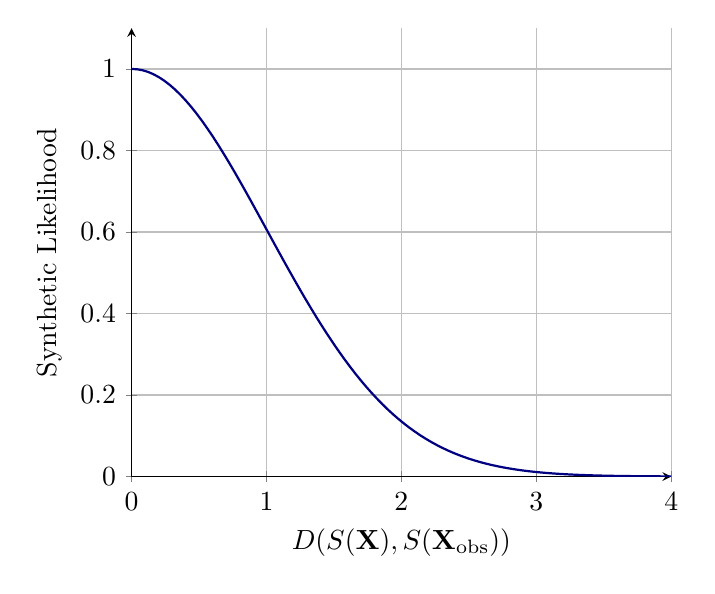
\begin{tikzpicture}
            \begin{axis}[
                    xlabel={$D(S(\mathbf{X}), S(\mathbf{X}_\text{obs}))$},
                    ylabel={Synthetic Likelihood},
                    xmin=0, xmax=4,
                    ymin=0, ymax=1.1,
                    domain=0:4,
                    samples=100,
                    axis lines=left,
                    grid=major,
                ]

                \addplot [blue!50!black, thick] {exp(-x^2/2)};

            \end{axis}
        \end{tikzpicture}
    \end{figure}
\end{frame}

\begin{frame}
    \frametitle{Attempt 2}
    \begin{figure}
        \centering
        \begin{tikzpicture}
        \begin{axis}[
            xlabel={$D(S(\mathbf{X}), S(\mathbf{X}_\text{obs}))$},
            ylabel={Synthetic Likelihood},
            xmin=0, xmax=2,
            ymin=0, ymax=1.1,
            axis lines=left,
            xtick={0.5},  % Define custom x tick at x = epsilon
            xticklabels={$\varepsilon$},  % Label the custom tick as epsilon
            % grid=major,
        ]

        % Plot y = 1 for 0 < x < epsilon
        \draw[blue!50!black, thick] (0,1) -- (0.5,1);

        % Plot y = 0 for x >= epsilon
        \draw[blue!50!black, very thick] (0.5,0) -- (2,0);

        % Mark epsilon
        \draw[dashed] (0.5,0) -- (0.5,1);

        \end{axis}
        \end{tikzpicture}
        \end{figure}


\end{frame}

\begin{frame}
    \frametitle{Overall Idea of my Research}
    \begin{itemize}
        \item What if we could 'predict' discrepency values we hadn't seen before?
        \item <2-> For parameters 'close' to parameters we've already tried it should be easy.
    \end{itemize}
\end{frame}

\begin{frame}
    \frametitle{Gaussian Processes}
    \begin{itemize}
        \item A class of random functions
        \item Common examples - Brownian motion, Ornstein Uhlenbeck process
        \item Model the mean discrepency using one of these (kriging)
    \end{itemize}
\end{frame}


\begin{frame}
    \frametitle{What choices do we have in a GP - correlation (length)}
    \includegraphics[width=\textwidth]{flatish_GP_ell_5_tenths.pdf}
    \end{itemize}
\end{frame}

\begin{frame}
    \frametitle{What choices do we have in a GP - correlation (length)}
    \includegraphics[width=\textwidth]{flatish_GP_ell_10_tenths.pdf}
    \end{itemize}
\end{frame}

\begin{frame}
    \frametitle{What choices do we have in a GP - correlation (length)}
    \includegraphics[width=\textwidth]{flatish_GP_ell_20_tenths.pdf}
    \end{itemize}
\end{frame}

\begin{frame}
    \frametitle{Sample frame title}

\end{frame}


\end{document}